\documentclass[0-protokol.tex]{subfiles}
\begin{document}

Hallův jev je důsledkem působení \textit{Lorentzovy síly} na náboje pohybující se v magnetickém poli. Na obrázku \ref{fig:vzorek} je znázorněn měřený vzorek germania. Kontakty 1 a 2 jsou \textit{proudové kontakty}, 3 a 4 jsou \textit{napěťové kontakty}, použité pro čtyřbodovou metodu měření. Kontakty 5 a 6 jsou určeny pro měření Hallova napětí.

\begin{figure}[H]
\centering
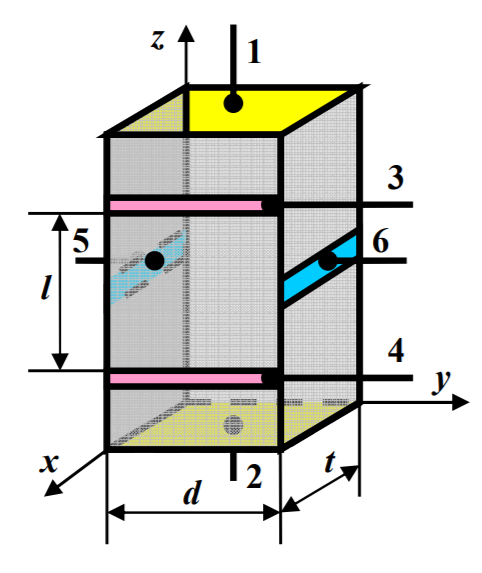
\includegraphics[scale=0.5]{vzorek}
\caption{Znázornění měřeného vzorku s rozměry a kontakty \cite{stud_text}}
\label{fig:vzorek}
\end{figure}

Vodivost vzorku při nulové magnetické indukci měříme pomocí zapojení \ref{fig:obvod1}. Platí vztah
\begin{equation} \label{eq:sigma}
\sigma = \frac{l}{td}\frac{I}{U} = \frac{lA}{td},
\end{equation}
kde $A$ dostaneme jako směrnici regresní přímky závislosti $I$ na $U$.

\begin{figure}[H]
\centering
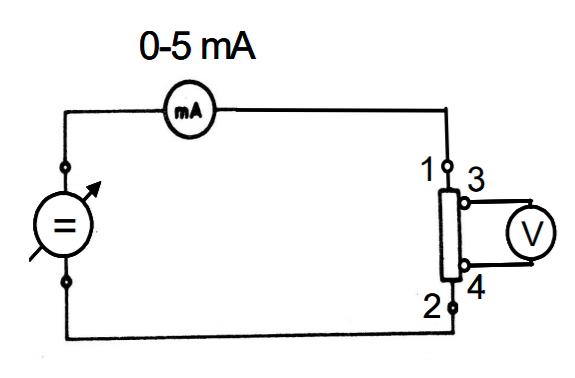
\includegraphics[scale=0.5]{obvod1}
\caption{Zapojení pro měření vodivosti \cite{stud_text}}
\label{fig:obvod1}
\end{figure}

Zapojení napájení elektromagnetu je vyobrazeno na obrázku \ref{fig:obvod2}. Intenzita magnetického pole souvisí s napájecím proudem vztahem
\begin{equation} \label{eq:indukce}
B = \num{0,098}I.
\end{equation}
Hallovo napětí měříme na svorkách 5 a 6 podle obrázku \ref{fig:vzorek}. Protože tyto svorky neleží na vzorku symetricky, měříme napětí při obou polaritách magnetické indukce. Hallovo napětí pak získáme jako 
\begin{equation} \label{eq:U_H}
|U_H| = \frac{|U^+ - U^-|}{2}.
\end{equation}

\begin{figure}[H]
\centering
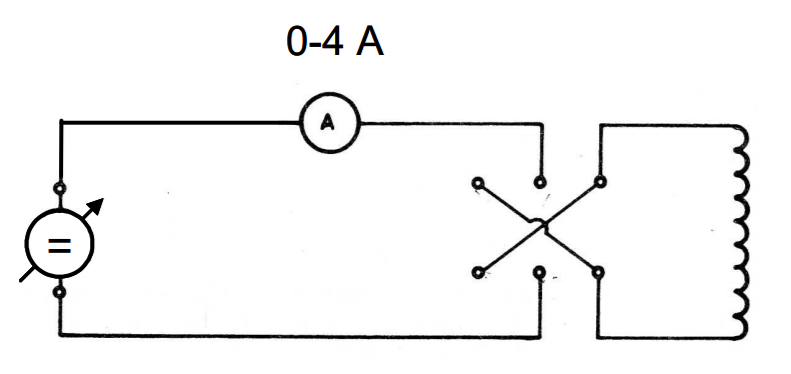
\includegraphics[scale=0.5]{obvod2}
\caption{Obvod pro napájení elektromagnetu \cite{stud_text}}
\label{fig:obvod2}
\end{figure}

Hallovu konstantu vzorku dostaneme ze vztahu
\begin{equation} \label{eq:R_H}
R_H = \frac{t U_H}{IB} = \frac{t C}{I},
\end{equation}
přičemž $C$ získáme jako směrnici regresní přímky závislosti $U_H$ na $B$.

Koncentraci nositelů náboje lze vyjádřit jako
\begin{equation} \label{eq:n}
n = \frac{r_h}{e R_H},
\end{equation}
kde $r_h = \frac{3 \pi}{8}$ je \textit{Hallův rozptylový faktor} \cite{stud_text} a $e \doteq \SI{1.6022e-19}{C}$ je \textit{elementární náboj} \cite{elem_naboj}.

Pohyblivost nositelů náboje dostaneme ze vztahu
\begin{equation} \label{eq:mu_n}
\mu_n = \frac{\sigma}{e n}.
\end{equation}

\end{document}
